\chapter{Metodología}

% \defaultFontEpigraph{Structured Pruning Is All You Need\dots}{\cite{caiStructuredPruningAll2022}}
\defaultFontEpigraph{Structured Pruning Is All You Need}{Cai y cols. (2022)}


\section{Revisión bibliográfica}

\subsection{Objetivos de la revisión}
La revisión bibliográfica en este trabajo tendrá como propósito contextualizar la investigación en un marco teórico, comprender el estado actual del \gls{dl} y los \gls{llm}, e identificar el estado del arte en cuanto al uso de estos sistemas para la generación de música en código de programación.

\subsection{Fuentes y búsqueda}
Para llevar a cabo esta revisión, se consultarán diversas bases de datos, revistas especializadas y conferencias de relevancia en el ámbito principalmente de la \gls{ia} y el prompting. La publicación de artículos científicos en el área de la \gls{ia}, y, en concreto, de \gls{llm}, es diaria, y debido a que la mayoría de estos trabajos han sido publicados durante 2022 y 2023, no cuentan con revisión por pares u otros mecanismos de verificación de las tesis en ellos contenidas. Por esta razón, sus resultados deben ser tomados con cautela y como líneas abiertas de investigación.


\subsection{Selección y evaluación}
Los criterios utilizados para seleccionar los trabajos incluidos en esta revisión se centraron en la relevancia y actualidad (véase la Figura \ref{fig:publications_per_year_referencias}), ya que la investigación en \gls{dl} se mueve a gran velocidad. Se dieron prioridad a trabajos publicados en los últimos meses y aquellos que se centran específicamente en aspectos cruciales de los \gls{llm} y la interacción mediante prompting y la generación de código de programación.

\begin{figure}[h]
    \caption[Publicaciones por año de las referencias utilizadas]{Publicaciones por año de las referencias utilizadas en este trabajo. Se observa un claro predominio de publicaciones relevantes especialmente en 2023.}
    \centering
    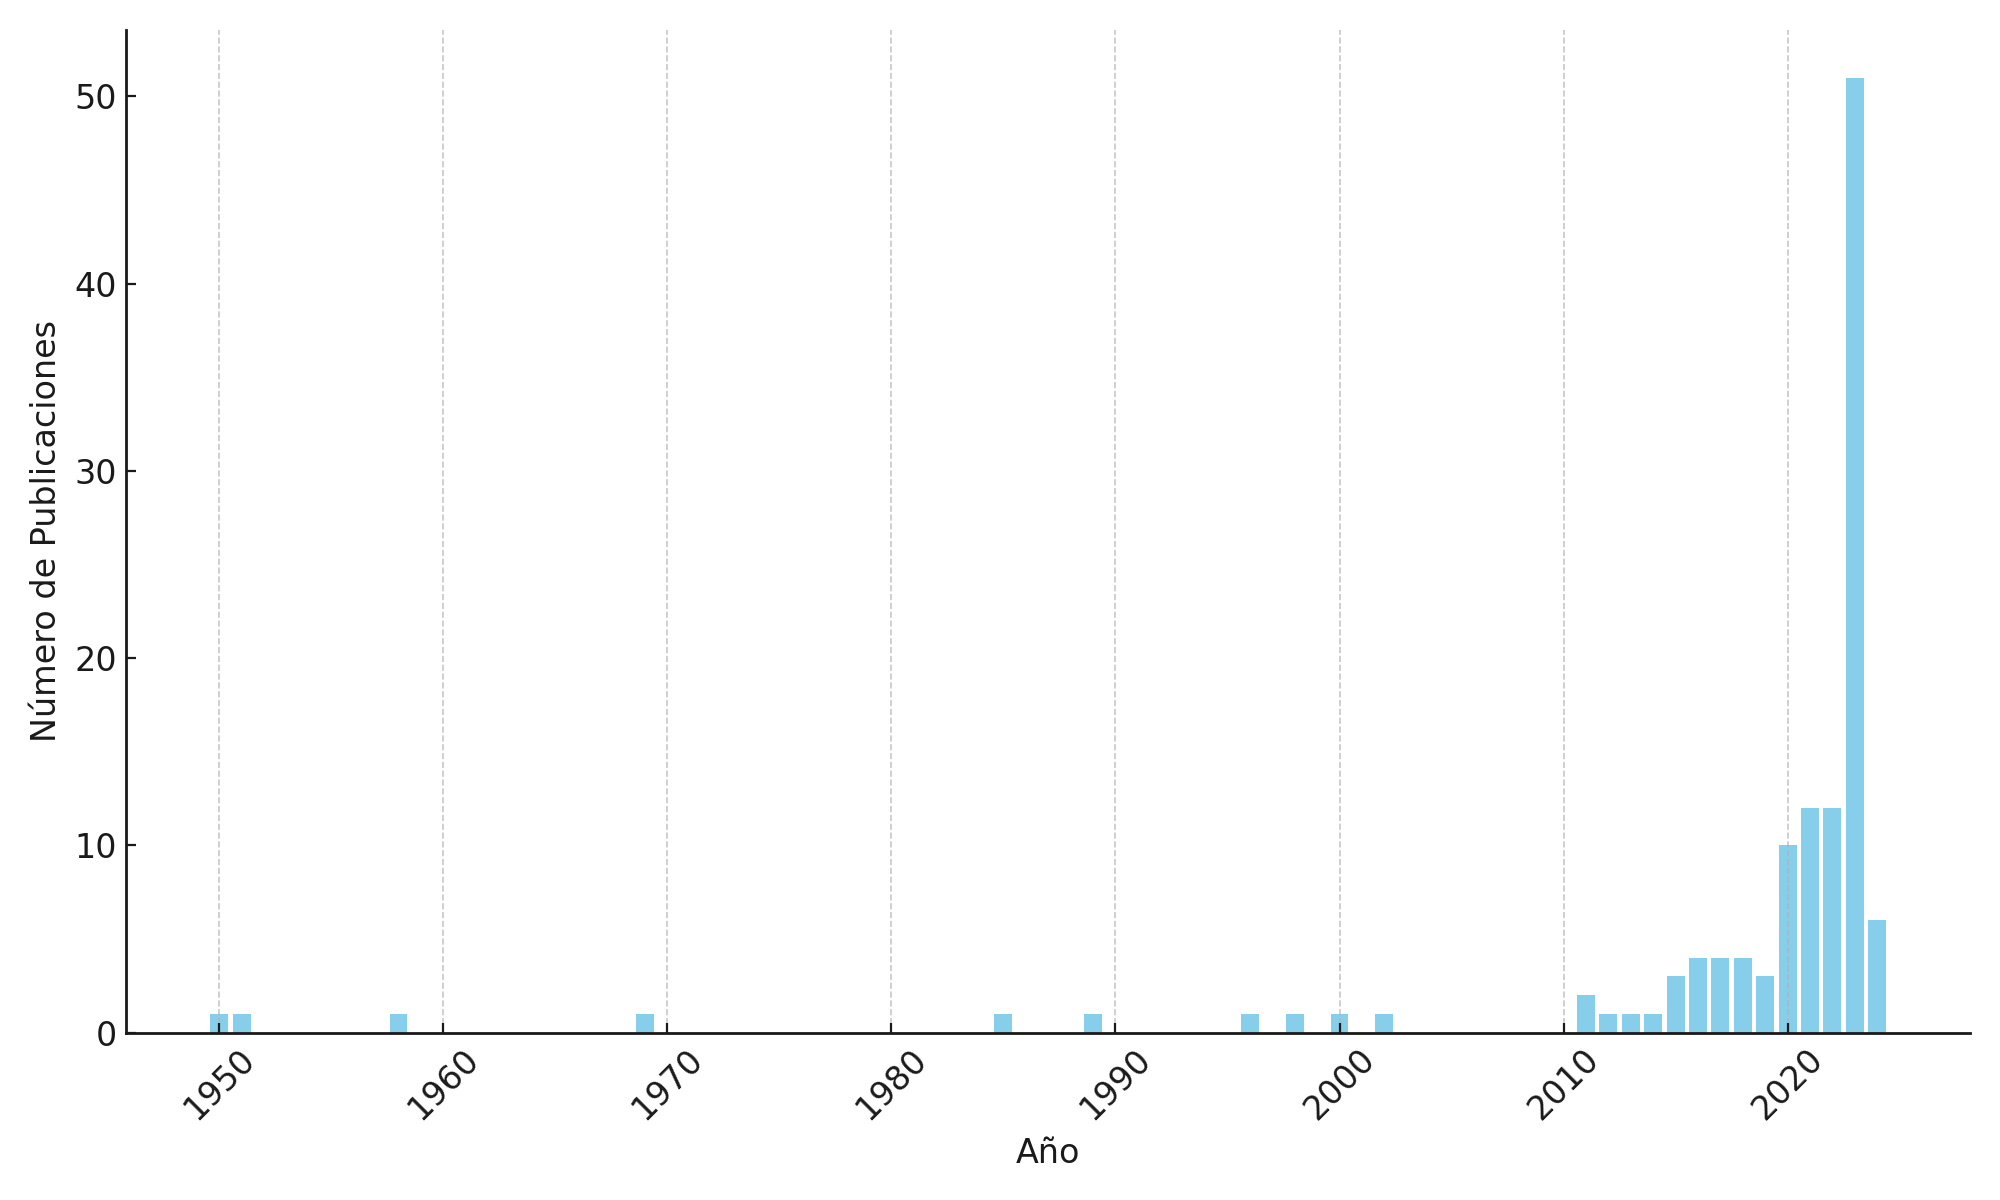
\includegraphics[width=0.7\textwidth]{./figuras/publications_per_year_referencias.png}
    \source{\propio}
    \label{fig:publications_per_year_referencias}
\end{figure}

Aunque la mayor parte de las referencias utilizadas han sido publicados en los últimos años, se han incluido algunos trabajos de referencia publicados en años anteriores, especialmente para conceptos clave en el campo de la \gls{ia} y el \gls{dl}.

\subsection{Resultados de la revisión}
Los hallazgos más relevantes de esta revisión son discutidos en detalle en la sección correspondiente al \hyperref[chap:estado_cuestion]{estado de la cuestión}. No obstante, es importante destacar que existen múltiples enfoques y técnicas para interactuar con los \gls{llm}, y que su aplicación en la composición musical aún se encuentra en una fase exploratoria, al no ser un objetivo primordial de los investigadores en el campo de la generación de código. Por otra parte, la mayoría de los trabajos publicados en el área de la música y los modelos generativos se centran en la generación de música como audio, y no en la interacción con los \gls{llm} como herramienta de composición. 

\section{Enfoque, alcance y diseño}

\subsection{Enfoque}

El enfoque de esta investigación es {cualitativo}, aunque se apoya en estudios previos de carácter cuantitativo. Será el propio investigador quien lleve a cabo la práctica y la evaluación de los resultados, con un claro acento en la reflexión sobre los procesos creativos implicados.

\subsection{Alcance}
La investigación tiene un alcance {exploratorio} y {descriptivo}. Es exploratorio en la medida en que se busca comprender y descubrir posibles aplicaciones de los \gls{llm} en el contexto de la composición musical algorítmica, un campo que aún no ha sido ampliamente estudiado. Al mismo tiempo, se adopta un enfoque descriptivo para detallar los resultados de la interacción con los sistemas de \gls{ia}.


\subsection{Diseño}
El diseño de esta investigación es {no estructurado}, en tanto que se sigue un plan abierto de actuación, por su naturaleza exploratoria, en función de los resultados de fases anteriores.

El trabajo tendrá un carácter {observacional}, donde el papel del investigador será el de observador y participante en el proceso de interacción creativa con sistemas de \gls{ia}.

\section{Herramientas y recursos utilizados}

Para llevar a cabo este estudio, se utilizarán ciertas herramientas informáticas:

\begin{enumerate}
    \item Ordenador personal con sistema operativo Linux.
    \item Visual Studio Code como editor de código.
    \item Python como lenguaje de programación.
    \item Diversos programas de síntesis de sonido, especialmente: SuperCollider, Tidal Cycles, Sonic Pi y Csound.
    \item \emph{Ardour} como \gls{daw}.
    \item Servicio de \emph{Advanced Data Analysis} de OpenAI para la elaboración de gráficas cuantitativas.
    \item Servicio de ChatGPT Plus y uso de la \gls{api} de OpenAI para la interacción con los \gls{llm}.
    \item Servicios de GitHub y Google Drive para el almacenamiento de datos.
\end{enumerate}


\section{Desarrollo y aplicación}

\subsection{Discusión de los criterios de elección de los lenguajes de programación musical}
En primer lugar se discutirán los criterios de elección de los lenguajes de programación musical utilizados en esta investigación: SuperCollider y Tidal Cycles. Se trata de una decisión importante, ya que el lenguaje de programación musical utilizado condicionará el tipo de interacción con los sistemas de \gls{llm}.

\subsection{Elección de los sistemas de \gls{llm} a utilizar}
Al mismo tiempo, y de forma relacionada con la elección de los lenguajes musicales, se discutirán las razones de la elección de los servicios de OpenAI para esta investigación.


\subsection{Exploración de posibles interfaces de interacción con sistemas de \gls{llm}}
De algún modo, esta será la guía de la investigación. A partir de las posibilidades  ofrecidas principalmente por OpenAI, se explorarán las posibilidades de interacción en la creación de código de programación musical, así como la calidad de los resultados que se obtengan aplicando diversas técnicas conocidas de prompting. Se comenzará con la interfaz más inmediata, que es el uso de chatbots, y se irá avanzando hacia el uso de la \gls{api} de OpenAI y la programación de scripts en Python.

% Seguir revisando por aquí.

\subsection{Documentación de las interacciones}
En cada fase de la investigación se guardarán los archivos de texto con las interacciones realizadas, los prompts utilizados, los resultados obtenidos y las reflexiones sobre el proceso.

\subsection{Creación de una pieza de arte sonoro}
Una vez exploradas diferentes interfaces de comunicación con sistemas de \gls{llm}, se procederá a la creación de una pieza de música algorítmica electroacústica que implique una interacción creativa con un sistema de \gls{llm}. La metodología concreta de composición se decidirá en función de los resultados obtenidos en las fases previas.

\subsection{Análisis cualitativo y reflexión}
En cada fase se procederá al análisis de los resultados obtenidos, dirigiendo así el proceso de investigación a pasos posteriores. Acabado todo el proceso experimental y de composición musical, se procederá a sintetizar los resultados y a realizar una reflexión final.

\subsection{Reflexión de las limitaciones y prospectivas}
Debido al carácter exploratorio de esta investigación, es necesario reflexionar sobre las limitaciones inherentes a la misma, así como discutir las posibles líneas de investigación futuras, especialmente hacia el diseño de investigaciones cuantitativas y de mayor alcance.

\subsection{Disponibilidad y publicación de los scripts del trabajo}
Todos los scripts utilizados en este trabajo, así como los prompts utilizados, códigos musicales obtenidos y el texto de esta memoria, quedarán almacenados y disponibles a la comunidad científica (véase anexo \ref{anexo:repositorio}).